\documentclass{article}

\usepackage[final]{neurips_2026}
\makeatletter
\renewcommand{\@notice}{}
\makeatother

\usepackage[utf8]{inputenc} % allow UTF-8 input
\usepackage[T1]{fontenc}    % use 8-bit T1 fonts
\usepackage[hidelinks]{hyperref} % hyperlinks without colored borders
\usepackage{url}            % simple URL typesetting
\usepackage{booktabs}       % professional-quality tables
\usepackage{amsmath}        % equations and aligned math
\usepackage{amsfonts}       % blackboard math symbols
\usepackage{graphicx}       % figures
\usepackage{nicefrac}       % compact fractions
\usepackage{microtype}      % microtypography
\usepackage{xcolor}         % colors

\title{Can Agents Learn When to Verify or Repair Memory Under Budget Constraints and Access Uncertainty?\\\large CMSC848N Midterm Report}
\author{%
  Arik Gershman \\
  Department of Computer Science \\
  University of Maryland\\
  \texttt{arikger@umd.edu}
  \And
  Shohini Rhea Sarkar \\
  Department of Computer Science \\
  University of Maryland\\
  \texttt{ssarkar6@terpmail.umd.edu}
  \And
  Amelia Harn \\
  Department of Computer Science \\
  University of Maryland\\
  \texttt{aharn1@umd.edu}
}

\begin{document}
\maketitle

\begin{abstract}
Long-running LLM agents store derived memories, such as summaries built from
many raw facts. When a fact is corrected, every summary built on it becomes
stale. Existing memory systems focus on detecting or invalidating outdated
facts but leave open what to do with stale summaries afterward. We study this
as an online rent-or-buy decision made at query time: VERIFY a stale summary
against current source facts for one query at a small cost, or REPAIR it once
at a larger cost that benefits all later queries, without knowing how often it
will be queried again. We have built a memory substrate (an append-only fact
ledger, summaries with exact provenance and transitive staleness, and hybrid
retrieval), seven runnable policies, a seeded workload generator, and an evaluator that scores each policy against a hindsight oracle. In
preliminary experiments on 10,000-memory synthetic workloads (5 seeds, two
demand mixes, three cost ratios, nominal costs), the classic threshold policy
P1 stays within 1.39--1.66$\times$ of the oracle in every setting, while
the eager, lazy, and verify-only baselines each exceed 2$\times$ in some
setting. A simple history-based predictor (P2) improves on P1 by up to 12\% at
high cost ratios. However, P1 loses to eager or first-access repair when most
memories are reused, so our first hypothesis holds only in part. We outline the remaining plan:
a repair budget, LLM-backed operations with measured costs, a learned demand
policy, held-out and shifting workloads, and a LongMemEval subset.
\end{abstract}

\section{Introduction}

LLM agents that run for weeks or months keep long-term memory in two layers:
raw records of what they have been told, and derived memories, such as
summaries, user profiles, and reflections, that are generated from those
records and retrieved at query time. Derived memories make retrieval cheaper
and answers more coherent, but they go out of date. When a user corrects a
fact (``I moved to Boston''), every summary built on the old value is wrong,
and the agent may keep answering from it.

Recent systems address the \emph{detection} side of this problem. Graphiti, the
engine behind Zep, stores facts in a temporal knowledge graph and invalidates
edges when newer information contradicts them~\citep{rasmussen2025zep};
All-Mem~\citep{lv2026allmem} and freshness-aware retrieval
methods~\citep{vectorize2026staleness} likewise track or down-weight outdated
content. What these systems leave open is what to do once staleness is known.
Rebuilding every affected derived memory as soon as a correction arrives wastes
work on memories that are never queried again. Checking the source records
every time a stale memory is used is cheap per query, but the memory is never
fixed, so a popular summary pays for the same check again and again.

We treat this as an online choice made at query time. When a query touches a
stale summary, the agent can VERIFY, consulting the current source facts to
answer this one query at cost $c_v$, or REPAIR, regenerating the summary at a
larger one-time cost $c_r$ that benefits every later query. If the summary will
be queried $k$ more times before its sources change again, repair is worth it
exactly when $k\,c_v > c_r$, but $k$ is unknown when the decision is made. This
is the rent-or-buy structure of ski rental~\citep{karlin1988snoopy}, which
gives simple policies with worst-case guarantees and a clear place where
learned predictions of reuse can help~\citep{purohit2018improving}.

\paragraph{Research question.} When a correction leaves part of a large memory
system potentially stale, can an agent decide at query time whether to
temporarily verify it or permanently repair it, under a limited maintenance
budget and without knowing how often that memory will be queried again?

\paragraph{Success criteria.} We test three hypotheses from the proposal.
\textbf{H1:} the threshold rule P1 never costs more than both Eager Refresh and
Verify-Only on any workload mix, and gives no more stale answers.
\textbf{H2:} a demand-aware policy comes closer to the hindsight oracle than P1
on warm and hot summaries. \textbf{H3:} under shifting demand, a hedged
demand-aware policy stays close to the oracle while a fully trusting one
degrades. The primary measurements are total maintenance cost $C(\pi)$, regret
$C(\pi)-C(\mathrm{oracle})$, the ratio $C(\pi)/C(\mathrm{oracle})$, the
stale-answer rate, and p95 query latency.

\paragraph{Scope.} We study the maintenance decision on its own. Memory layout,
staleness propagation, retrieval, and the verify/repair implementation are held
fixed across policies, so measured differences come from the policy alone.
Section~\ref{sec:prelim} reports controlled synthetic experiments at 10K
memories with deterministic operations; LLM-backed operations, a repair budget,
and benchmark evaluation are planned (Section~\ref{sec:plan}).

\section{Related Work}

\paragraph{Online rent-or-buy decisions.} Verify-versus-repair parallels the
ski-rental problem: keep paying a small recurring cost or pay a large one-time
cost, without knowing the horizon. \citet{karlin1988snoopy} introduced the
deterministic threshold strategy, which pays at most twice the hindsight
optimum, and \citet{karlin1994randomized} gave a randomized strategy with
expected ratio about $e/(e-1)\approx1.58$. \citet{purohit2018improving} add a
machine-learned prediction of the horizon and a trust parameter that trades
consistency (near-optimal when predictions are good) against robustness
(bounded loss when they are wrong). Our P1 is the classic deterministic rule
applied per stale episode; our planned P3 follows the Purohit et al.\ structure
with a learned estimate of future accesses. \citet{li2025combinatorial} extend
ski rental to bundles of items, which may inform repairing related summaries
together. Unlike these analyses, our ``horizon'' is a memory's future query
count, which is observable only through past accesses, and many items share
one maintenance budget.

\paragraph{Knowledge editing.} ROME and MEMIT locate factual associations in
feed-forward layers and edit them with targeted
updates~\citep{meng2022rome,meng2023memit}. They correct the edited fact but
not conclusions that depend on it; EchoEdit~\citep{shi2026echoedit} edits
semantically related nodes to control these ripple effects. We study the same
dependency problem in external memory, where dependencies are explicit
(provenance links) and the question is \emph{when} a dependent memory is worth
fixing rather than \emph{how} to fix it.

\paragraph{Memory systems for long-running agents.} Zep/Graphiti keeps a
bitemporal knowledge graph and invalidates contradicted
edges~\citep{rasmussen2025zep}. All-Mem performs lightweight online writes and
defers SPLIT/MERGE/UPDATE reorganization to an offline LLM
phase~\citep{lv2026allmem}. MemStrata-style temporal validity
fields~\citep{yadav2026memstrata} inspired our append-only ledger.
LongMemEval~\citep{wu2025longmemeval} and
LongMemEval-V2~\citep{wu2026longmemevalv2} benchmark recall over long
histories, including knowledge updates. These systems detect or route around
stale content; none decides per memory whether repair is worth its cost given
uncertain reuse.

\paragraph{Baselines.} From this literature and common practice we derive
five runnable baselines, all implemented: \emph{Verify-Only} (never repair),
\emph{Eager Refresh} (repair every affected summary at correction time, the
invalidate-and-rebuild default), \emph{Repair-on-First-Access} (lazy rebuild),
\emph{Periodic Refresh} (scheduled batch rebuild, analogous to offline
reorganization in All-Mem), and \emph{Oldest-First} (bounded background repair
by stale age). The \emph{hindsight oracle}, which knows each memory's future
query count, gives the lower bound used for regret.

\section{Methodology}

\subsection{Problem formulation}
A \emph{stale episode} for summary $s$ runs from the correction that marks it
stale until it is repaired or a later correction starts a new episode. Let
$k_s$ be the number of queries that reach $s$ during the episode. On each such
query the policy chooses VERIFY or REPAIR; after a repair, the remaining
queries use the fresh summary at no maintenance cost. A policy $\pi$ is scored by
\begin{equation}
C(\pi) = c_v N_v(\pi) + c_r N_r(\pi) + \lambda N_{\mathrm{stale}}(\pi),
\label{eq:cost}
\end{equation}
where $N_v$ and $N_r$ count verifications and repairs and $N_{\mathrm{stale}}$
counts answers that used outdated facts. In hindsight the best cost for an
episode is $\min(k_s c_v,\, c_r)$: verify every query, or repair on the first.
We report results in terms of the ratio $\rho=c_r/c_v$.

\subsection{Memory substrate}
\textbf{Source fact ledger.} An append-only SQLite table: each record stores
entity, attribute, value, validity interval, version, and the record it
supersedes. Corrections, real updates, retractions (immutable tombstones), and
temporary exceptions (which expire and restore the prior value) are all new
rows; existing rows are never updated or deleted. Current and historical values
are resolvable at any timestamp.
\textbf{Derived summary store.} Each summary records the exact fact versions it
was built from; a reverse index maps each fact to dependent summaries, and
summary-to-summary dependencies form a DAG. A correction marks direct and
transitive dependents stale and starts a new stale episode, with counters for
verifications and spending in the episode.
\textbf{Retrieval.} SQLite FTS5 keyword search, BGE-M3~\citep{chen2024bgem3}
dense search over FAISS~\citep{douze2024faiss}, and reciprocal rank
fusion~\citep{cormack2009rrf}.

\subsection{Maintenance operations}
VERIFY resolves the current version of each source fact and returns it as
evidence for this query; the stored summary, its provenance, and its stale flag
are unchanged. REPAIR rebuilds the summary from current facts, updates its
provenance and retrieval indexes, and clears the stale flag in one SQLite
transaction (the semantic index is rebuilt if the transaction fails). In the
current prototype both operations are deterministic (template rebuild), so
costs are nominal; Section~\ref{sec:plan} describes the planned LLM-backed
versions.

\subsection{Policies}
Policies only return decisions; the simulator validates and executes them.
\textbf{P1 (accumulated threshold)} verifies on the first $m-1$ queries of an
episode and repairs on query $m=\lceil c_r/c_v\rceil$, computed exactly on the
decimal cost values. Per episode it costs at most
$(m-1)c_v+c_r<2\cdot\mathrm{OPT}$ when $k_s\ge m$, and exactly OPT otherwise.
\textbf{P2 (predicted threshold)} maintains, per summary, an exponentially
decayed access count (half-life 1\,h) over \emph{completed} past accesses,
including accesses while fresh. It forecasts additional accesses over a 24\,h
rolling horizon and repairs immediately when the current query plus the
forecast would cost at least one repair. The forecast is used only when it is
``confident'' (at least 3 past accesses, the last within one half-life, and a
decayed count of at least 1.5); otherwise P2 behaves exactly like P1. This is a
hedged variant of the proposal's P2: a low forecast never delays repair beyond
P1's threshold. Policies never receive future accesses or group labels.

\subsection{Synthetic workloads and evaluation}
The generator creates people, projects, and places; each memory is one summary
over three facts. Every memory receives exactly one correction, and all
corrections precede all queries. Each memory is assigned to a demand group with
an exact future query count drawn uniformly from cold (0--2), warm (3--10), or
hot (11--50); queries are then shuffled with a seeded RNG. Each query names a
unique entity, so keyword retrieval always reaches the intended memory; this
deliberately removes retrieval error so that cost differences come from
maintenance decisions. The workload file stores the true future counts as
evaluator-only metadata. After each replay the evaluator computes per-memory
cost from the logs, checks that each memory received exactly its recorded
query count, and compares against $\sum_s \min(k_s c_v, c_r)$. The oracle was
validated against exhaustive search over all action sequences for
$k\le7$ and several cost pairs.

\section{Preliminary Experiments and Results}
\label{sec:prelim}

\subsection{What was run}
\textbf{Prototype.} The full substrate above is implemented in Python with
SQLite, together with seven runnable policies (five baselines, P1, P2), a
replayable simulator, the synthetic generator, and the oracle evaluator
(repository: \url{https://github.com/shohinirheasarkar/ShouldAgentsVerifyOrRepair}).
A suite of 348 pytest tests covers ledger immutability, temporal
resolution, provenance, transitive staleness, VERIFY non-mutation, atomic
REPAIR, P1/P2 switching boundaries, deterministic replay, and
the oracle (checked against exhaustive search). A toy end-to-end scenario
(``Alice lives in Maryland'' corrected to Boston) behaves as specified under
every policy.

\textbf{Experiment.} We generated 10,000-memory workloads with seeds 1--5 in
two demand mixes: \emph{balanced} (3,334 cold / 3,333 warm / 3,333 hot;
125.6K--127.6K queries per trace) and \emph{cold-heavy} (8,000 / 1,000 / 1,000;
44.4K--45.9K queries). Every policy replayed each saved trace at
$c_v=1$ and $c_r\in\{2,5,10\}$: 7 policies $\times$ 3 ratios $\times$ 5 seeds
$=105$ replays per mix. Scheduled baselines used one tick per 100 processed
events and Oldest-First one repair slot per tick. P2 used its defaults
(half-life 1\,h, horizon 24\,h, minimum 3 accesses). We report means over seeds
with 95\% Student-$t$ intervals. Costs are \emph{nominal units}, not
measurements. For the balanced mix we also recorded wall-clock latency per
query, from retrieval through any query-time VERIFY/REPAIR, on a MacBook
(8 cores, Python 3.12, five seeds as concurrent processes).

\subsection{Results}

\begin{table}[t]
\centering
\small
\caption{Cost relative to the hindsight oracle, $C(\pi)/C(\mathrm{oracle})$
(mean $\pm$ 95\% CI over 5 seeds, 10K memories). Lower is better; 1.00 is
optimal. Bold marks the best non-oracle policy in each column. Oracle cost
(nominal units) is shown in the last row.}
\label{tab:main}
\begin{tabular}{@{}lcccccc@{}}
\toprule
 & \multicolumn{3}{c}{Balanced mix} & \multicolumn{3}{c}{Cold-heavy mix} \\
\cmidrule(lr){2-4}\cmidrule(lr){5-7}
Policy & $\rho=2$ & $\rho=5$ & $\rho=10$ & $\rho=2$ & $\rho=5$ & $\rho=10$ \\
\midrule
Verify-Only            & 7.61{\scriptsize$\pm$.05} & 3.57{\scriptsize$\pm$.03} & 2.17{\scriptsize$\pm$.02} & 3.77{\scriptsize$\pm$.04} & 2.57{\scriptsize$\pm$.03} & 1.84{\scriptsize$\pm$.03} \\
Eager Refresh          & 1.20{\scriptsize$\pm$.00} & 1.41{\scriptsize$\pm$.00} & 1.71{\scriptsize$\pm$.00} & 1.67{\scriptsize$\pm$.02} & 2.85{\scriptsize$\pm$.02} & 4.08{\scriptsize$\pm$.01} \\
Repair-on-First-Access & \textbf{1.07}{\scriptsize$\pm$.00} & \textbf{1.25}{\scriptsize$\pm$.00} & 1.52{\scriptsize$\pm$.01} & \textbf{1.22}{\scriptsize$\pm$.01} & 2.08{\scriptsize$\pm$.01} & 2.98{\scriptsize$\pm$.01} \\
Periodic Refresh       & 1.20{\scriptsize$\pm$.00} & 1.41{\scriptsize$\pm$.00} & 1.71{\scriptsize$\pm$.00} & 1.67{\scriptsize$\pm$.02} & 2.85{\scriptsize$\pm$.02} & 4.08{\scriptsize$\pm$.01} \\
Oldest-First           & 7.20{\scriptsize$\pm$.06} & 3.50{\scriptsize$\pm$.03} & 2.24{\scriptsize$\pm$.02} & 3.74{\scriptsize$\pm$.04} & 2.64{\scriptsize$\pm$.03} & 2.01{\scriptsize$\pm$.03} \\
P1 (threshold)         & 1.47{\scriptsize$\pm$.00} & 1.66{\scriptsize$\pm$.00} & 1.58{\scriptsize$\pm$.00} & 1.39{\scriptsize$\pm$.00} & 1.40{\scriptsize$\pm$.00} & 1.41{\scriptsize$\pm$.01} \\
P2 (predicted)         & 1.47{\scriptsize$\pm$.00} & 1.64{\scriptsize$\pm$.00} & \textbf{1.42}{\scriptsize$\pm$.00} & 1.39{\scriptsize$\pm$.00} & \textbf{1.35}{\scriptsize$\pm$.00} & \textbf{1.24}{\scriptsize$\pm$.01} \\
\midrule
Oracle cost            & 16,640 & 35,417 & 58,357 & 11,956 & 17,578 & 24,485 \\
\bottomrule
\end{tabular}
\end{table}

\begin{figure}[t]
\centering
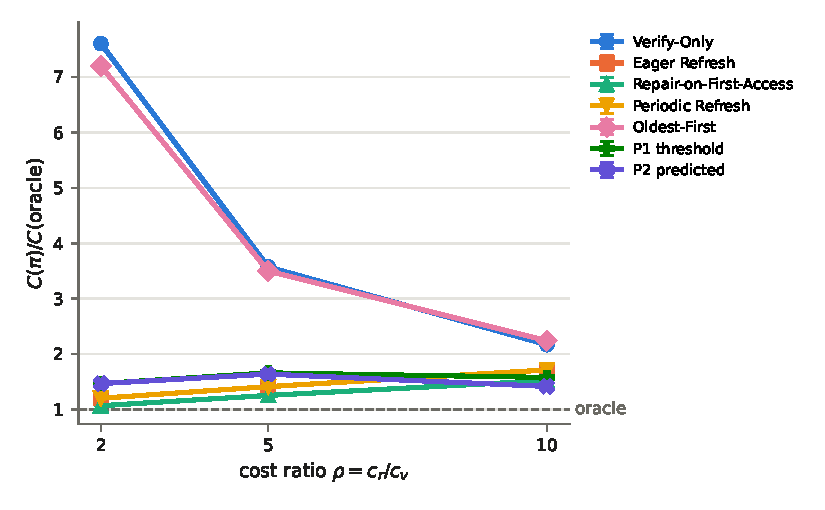
\includegraphics[width=0.49\linewidth]{figures/balanced/cost_vs_ratio.pdf}\hfill
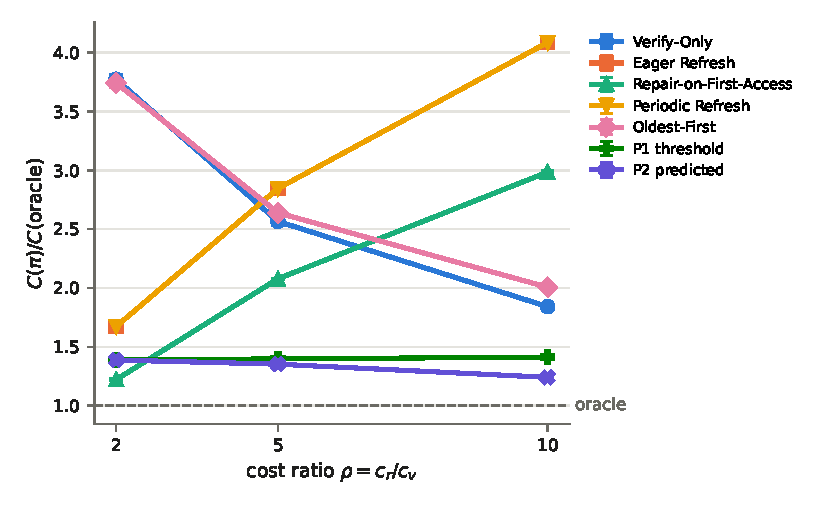
\includegraphics[width=0.49\linewidth]{figures/cold-heavy/cost_vs_ratio.pdf}
\caption{$C(\pi)/C(\mathrm{oracle})$ versus $\rho=c_r/c_v$ for the balanced
(left) and cold-heavy (right) mixes; error bars are 95\% CIs (most are smaller
than the markers). Eager Refresh and Periodic Refresh coincide exactly (see
text). Values are in Table~\ref{tab:main}.}
\label{fig:ratio}
\end{figure}

\begin{figure}[t]
\centering
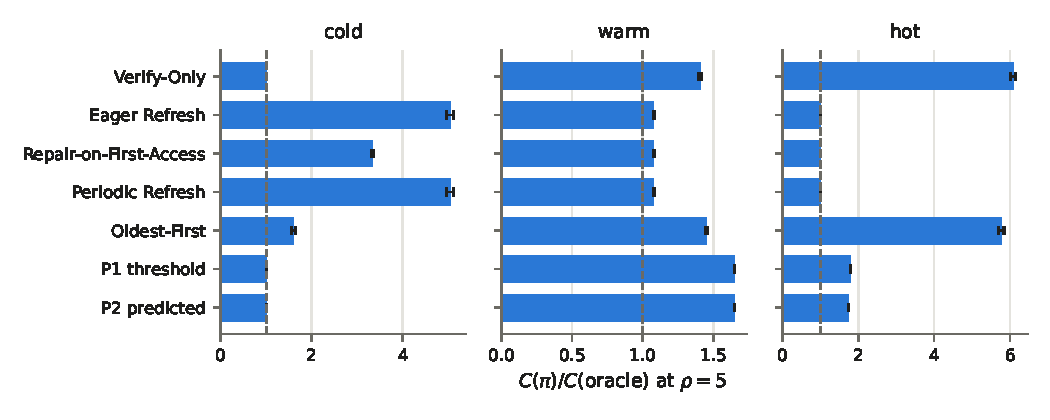
\includegraphics[width=0.9\linewidth]{figures/balanced/cost_by_group.pdf}
\caption{Balanced mix at $\rho=5$: $C(\pi)/C(\mathrm{oracle})$ within each
demand group (note the different x-axis scales). Eager and first-access repair
waste repairs on cold memories; Verify-Only pays heavily on hot ones; P1 and P2
are exact on cold memories and pay a bounded premium on warm and hot ones.}
\label{fig:groups}
\end{figure}

Table~\ref{tab:main} and Figure~\ref{fig:ratio} give the main results;
Figure~\ref{fig:groups} breaks the balanced mix down by demand group.

\textbf{The rent-or-buy tradeoff appears as expected.} Verify-Only is optimal on
cold memories (ratio 1.00) and worst on hot ones (6.09 at $\rho=5$); Eager
Refresh is optimal on hot memories and worst on cold ones (5.04). In the
cold-heavy mix the two cross between $\rho=2$ and $\rho=5$: Eager Refresh is
cheaper at $\rho=2$ and Verify-Only at $\rho\ge5$.

\textbf{P1 is the most robust policy without prediction.} Its ratio stays
between 1.39 and 1.66 in all six settings, while every baseline exceeds 2.9
in at least one setting. Within every group P1 stays below its theoretical
worst case of 2; the largest value, 1.90 on hot memories at $\rho=10$, equals
the per-episode bound $2-1/m$ exactly. It never answers from a
stale source and is always cheaper than Verify-Only.

\textbf{H1 holds only in part.} P1 is cheaper than both Eager Refresh and
Verify-Only in four of six settings, but in the balanced mix at $\rho=2$ and
$\rho=5$ it costs more than Eager Refresh (24.4K vs.\ 20.0K and 58.8K vs.\
50.0K). The balanced mix has 89\% of memories queried at least once and two
thirds queried three or more times, so repairing early is almost always right,
and P1 pays its $(m-1)$ verifications before every repair. On this mix,
Repair-on-First-Access is the best practical policy at $\rho\le5$. As the
proposal intended, H1 should be read as a statement about robustness across
mixes, and our results support it in that form. In its strict
per-workload form it is false.

\textbf{Prediction helps only once a memory has enough history.} P2 matches P1
exactly at $\rho=2$: it needs three completed accesses before its forecast is
trusted, and P1 already repairs on the second. The gain grows with $\rho$
(balanced: 1.66$\to$1.64 at $\rho=5$, 1.58$\to$1.42 at $\rho=10$;
cold-heavy: 1.40$\to$1.35 and 1.41$\to$1.24), and almost all of it comes from hot
memories, whose accesses are close enough together for the recency gate to
pass (hot, $\rho=10$: 1.90$\to$1.60 balanced, 1.90$\to$1.36 cold-heavy). The
forecast is not free: on \emph{warm} memories at $\rho=10$, P2 is worse than
P1 (1.17$\to$1.19 balanced, 1.17$\to$1.36 cold-heavy), because a short burst
of accesses can trigger an early repair for a memory that is then queried only
a few more times. P2's total cost was never above P1's in any setting. This is
preliminary evidence for H2's premise from a simple non-learned predictor, and
an early example of the robustness concern behind H3.

\textbf{Background repair with a small schedule budget behaves like Verify-Only.}
Oldest-First made only 551--1,365 repairs (one per 100 events). Because
stale age reflects correction order, not demand, those repairs fall evenly
across groups, including cold memories that are never queried again (ratio 1.6 on cold at $\rho=5$).
This motivates ranking deferred repairs by predicted savings, as the proposal's
budget design does.

\begin{table}[t]
\centering
\small
\caption{Wall-clock query latency (ms) on the balanced mix at $\rho=5$, mean
over 5 seeds of each seed's percentile. ``Maint.''\ = queries that performed
VERIFY or REPAIR. Deterministic operations only: these are not LLM latencies.}
\label{tab:latency}
\begin{tabular}{@{}lrrrrr@{}}
\toprule
Policy & p50 & p95 & p99 & p95 maint. & p95 no maint. \\
\midrule
Verify-Only            & 0.31 & 0.73 & 1.02 & 0.73 & --- \\
Eager Refresh          & 0.18 & 0.43 & 0.59 & ---  & 0.43 \\
Repair-on-First-Access & 0.24 & 2.12 & 3.24 & 4.94 & 0.57 \\
Periodic Refresh       & 0.18 & 0.44 & 0.67 & ---  & 0.44 \\
Oldest-First           & 0.33 & 0.75 & 0.90 & 0.76 & 0.51 \\
P1                     & 0.26 & 1.12 & 2.39 & 2.24 & 0.55 \\
P2                     & 0.28 & 1.48 & 2.70 & 2.36 & 0.63 \\
\bottomrule
\end{tabular}
\end{table}

\textbf{Latency.} Table~\ref{tab:latency} shows the expected pattern: policies
that repair at query time move cost onto the user-visible path (RoFA's p95 is
2.1\,ms versus 0.43\,ms for Eager Refresh, which repairs in the background).
In this substrate a query-time REPAIR (index update) has a p95 near 5\,ms,
against 0.73\,ms for VERIFY (Verify-Only), a p95 ratio of about 7 for
deterministic operations. These numbers come
from template operations on a laptop with concurrent processes; they validate
the instrumentation, not the LLM cost model.

\subsection{Limitations and uncertainty}
\begin{itemize}
\item \textbf{Nominal costs.} $c_v$ and $c_r$ are assumed constants, and
VERIFY/REPAIR are deterministic templates; no LLM has been run. Conclusions
about which policy wins depend on $\rho$, which we have not yet measured for
LLM operations.
\item \textbf{Simplified workloads.} Each memory has exactly one correction,
before all queries, and three facts; queries are uniformly shuffled. Hence
Periodic Refresh repairs everything before the first query and is identical
to Eager Refresh, and no policy ever answers from a stale source (stale-answer
rate 0), so the $\lambda$ term in Eq.~\ref{eq:cost} is untested.
\item \textbf{Workload dependence.} The best practical policy changes with
the mix (Table~\ref{tab:main}); two mixes are not a sweep.
\item \textbf{No retrieval error.} Each query names a unique entity, so
retrieval always reaches the right memory. This isolates the policy
but overstates how well real systems would perform.
\item \textbf{Development data only.} All runs use seeds 1--5, and P2's
settings were chosen during development; there is no held-out evaluation yet.
CIs reflect seed-to-seed variation within one generator, not uncertainty
about other workloads.
\item \textbf{Not yet implemented:} the repair budget $B$, P3, the semantic
dirty-bit check, the randomized P1 variant, and benchmark evaluation.
\end{itemize}

\section{Evaluation Plan and Milestones}
\label{sec:plan}

\subsection{Tasks, data, and fair comparison}
\textbf{Controlled synthetic workloads (primary).} We will extend the generator
along the axes the preliminary results show matter: (i) corrections spread
through the trace (a Poisson process) and repeated corrections, so a memory
has several stale episodes and scheduled baselines are exercised; (ii) the
cold/warm/hot mix; (iii) $d$, the number of facts per summary, and dependency
fan-out; and (iv) \emph{shifting} demand, where memories move between groups
partway through the trace. Every policy replays the identical saved trace, cost
setting, and initial state; only the policy changes.

\textbf{Held-out protocol.} All results in this report use seeds 1--5 and are
treated as \emph{development} data; the P2 settings were chosen during
development. For the final evaluation we will freeze all policy settings,
train P3 only on training seeds, tune on separate development seeds, and report
on held-out test seeds not used before, plus a shift-test set whose group
assignments and shift schedule P3 never saw.

\textbf{Real-history benchmark (secondary).} We will adapt the knowledge-update
and temporal-reasoning questions of LongMemEval~\citep{wu2025longmemeval}:
sessions supply source facts, a corrected value starts a stale episode, and
later questions about the entity are accesses. Examples without a clear
correction-to-question mapping will be excluded, and benchmark results will
be reported separately from synthetic results. RealTime QA~\citep{kasai2023realtimeqa}
moves to a stretch goal.

\textbf{Metrics.} Total cost $C(\pi)$ (Eq.~\ref{eq:cost}) with measured
$c_v,c_r$; regret and $C(\pi)/C(\mathrm{oracle})$ by group; verification and
repair counts; stale-answer rate; p50/p95/p99 query latency separated into
queries with and without maintenance; and, once LLM operations exist, exact
match and token F1 on synthetic questions and official metrics on LongMemEval.
With a repair budget $B$ we report cost at fixed budget and the
budget-versus-cost curve against a budget-aware oracle (exact knapsack at 10K;
greedy by savings per unit cost at larger scales). Each setting uses at least
five seeds with 95\% confidence intervals; policy comparisons are paired on
identical traces.

\subsection{Compute and other budgets}
Deterministic replay needs only a laptop: one 10K replay takes about
45--75\,s, so a full 105-run grid takes about 25 minutes with five parallel
processes; we expect 100K replays to take roughly 10 minutes each. LLM-backed VERIFY/REPAIR will
use Qwen~2.5~7B Instruct~\citep{qwen2024qwen25} or Llama~3.1~8B
Instruct~\citep{grattafiori2024llama3}, 4-bit quantized, on Google Colab and
the group's RTX~5070 (12\,GB), with UMD's Zaratan cluster as a fallback. Running every
operation through an LLM at 10K (about 126K queries per trace) is too slow
for our hardware, so we will run LLM-in-the-loop experiments at 1K memories and
on the benchmark subset, record per-operation GPU time and tokens, and replay
those measured cost distributions at 10K and 100K (the proposal's cost-replay
mode). We no longer plan hosted-API text generation; template text is
sufficient for the policy experiments, so the API budget is zero.

\subsection{Risks and mitigations}
\begin{itemize}
\item \textbf{LLM integration has not started.} It is the main dependency for
measured costs, the semantic dirty-bit check, and answer quality. We will build
it first, at 1K scale; if it slips, we will report policy results under several
assumed ratios $\rho$ and measured costs only for the toy dataset.
\item \textbf{Conclusions depend on the workload.} Repair-on-First-Access is
the best practical policy on the balanced mix at $\rho\le5$ but among the
worst on the cold-heavy mix at $\rho\ge5$ (Section~\ref{sec:prelim}). We will
sweep the cold/warm/hot mix and the correction rate rather than report a single
workload.
\item \textbf{Prediction may add little.} P2 helps only once a memory has
enough history. P3 may not beat P1 or Repair-on-First-Access; we will report
that as a finding and include the hedged variant, which bounds the damage.
\item \textbf{Benchmark mapping.} Public benchmarks do not expose future access
counts or repeated reuse of a summary. If the mapping is too thin, the
benchmark will be used only to check answer quality, not to compare costs.
\end{itemize}

\subsection{Milestones}
Table~\ref{tab:milestones} gives the remaining schedule. Week~12 includes the
artifact audit; Week~15 is reserved for analysis and writing.

\begin{table}[h]
\centering
\small
\caption{Remaining milestones (target date is the end of each block).}
\label{tab:milestones}
\begin{tabular}{@{}p{0.13\linewidth}p{0.47\linewidth}p{0.32\linewidth}@{}}
\toprule
Weeks (target) & Tasks & Deliverable \\
\midrule
10 (Nov 8) & Repair budget $B$ with deferred-repair queue; budget-aware oracle; corrections spread over time, repeated corrections; Periodic Refresh that answers from stale summaries & Budget-vs-cost curves; stale-answer rate for scheduled baselines \\
11 (Nov 15) & LLM-backed VERIFY/REPAIR (4-bit 7--8B model); measured $c_v$, $c_r$ at 1K; cost-replay mode; semantic dirty-bit check at toy/1K scale & Measured cost distributions; flag precision \\
12 (Nov 22) & P3 (gradient-boosted trees~\citep{chen2016xgboost}) and its hedged variant on train/dev/test seeds; shifting workloads; artifact audit (CI, \texttt{pip-audit}, prompt-injection test) & P3 vs.\ P1/P2 on held-out and shifted traces; audit \\
13--14 (Dec 6) & LongMemEval subset; 100K cost-replay runs; repository cleanup; paper draft & Answer quality; 100K results; draft \\
15 (Dec 11) & Final analysis, paper, and slides & Final report and presentation \\
\bottomrule
\end{tabular}
\end{table}

\bibliographystyle{plainnat}
\bibliography{references}

\end{document}
